% Integration strategy section, to be included in iit.tex

\subsubsection{Integration strategy}
The implementation order has been developed considering the possibility to immediately integrate components and test their interactions; this way development time can be optimized even more and errors can be found as early as possible. The integration strategy is shown in the following figures.

\begin{figure}[h]
	\begin{subfigure}{.42\textwidth}
		\centering
		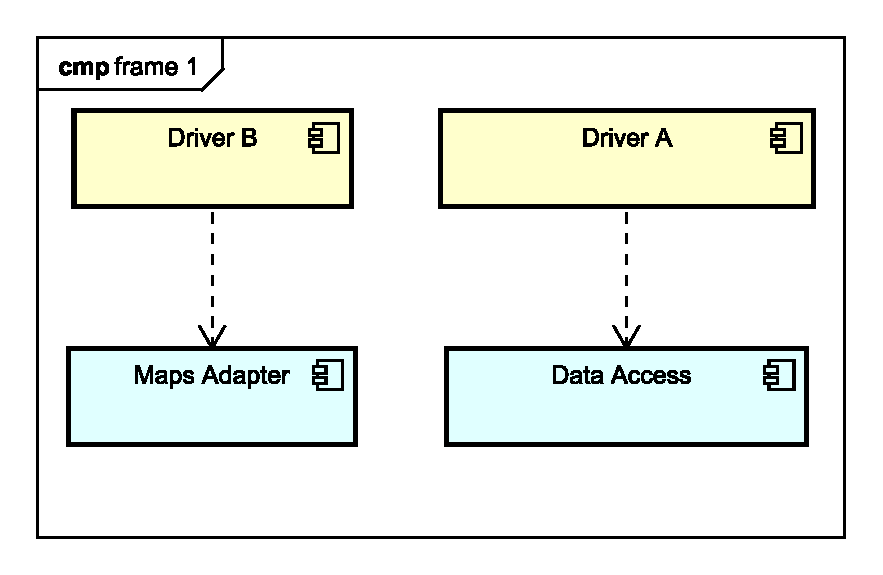
\includegraphics[width=\linewidth]{iit/frame_1}
		\caption{First components with their drivers}
		\label{frame_1}
	\end{subfigure}
	\begin{subfigure}{.58\textwidth}
		\centering
		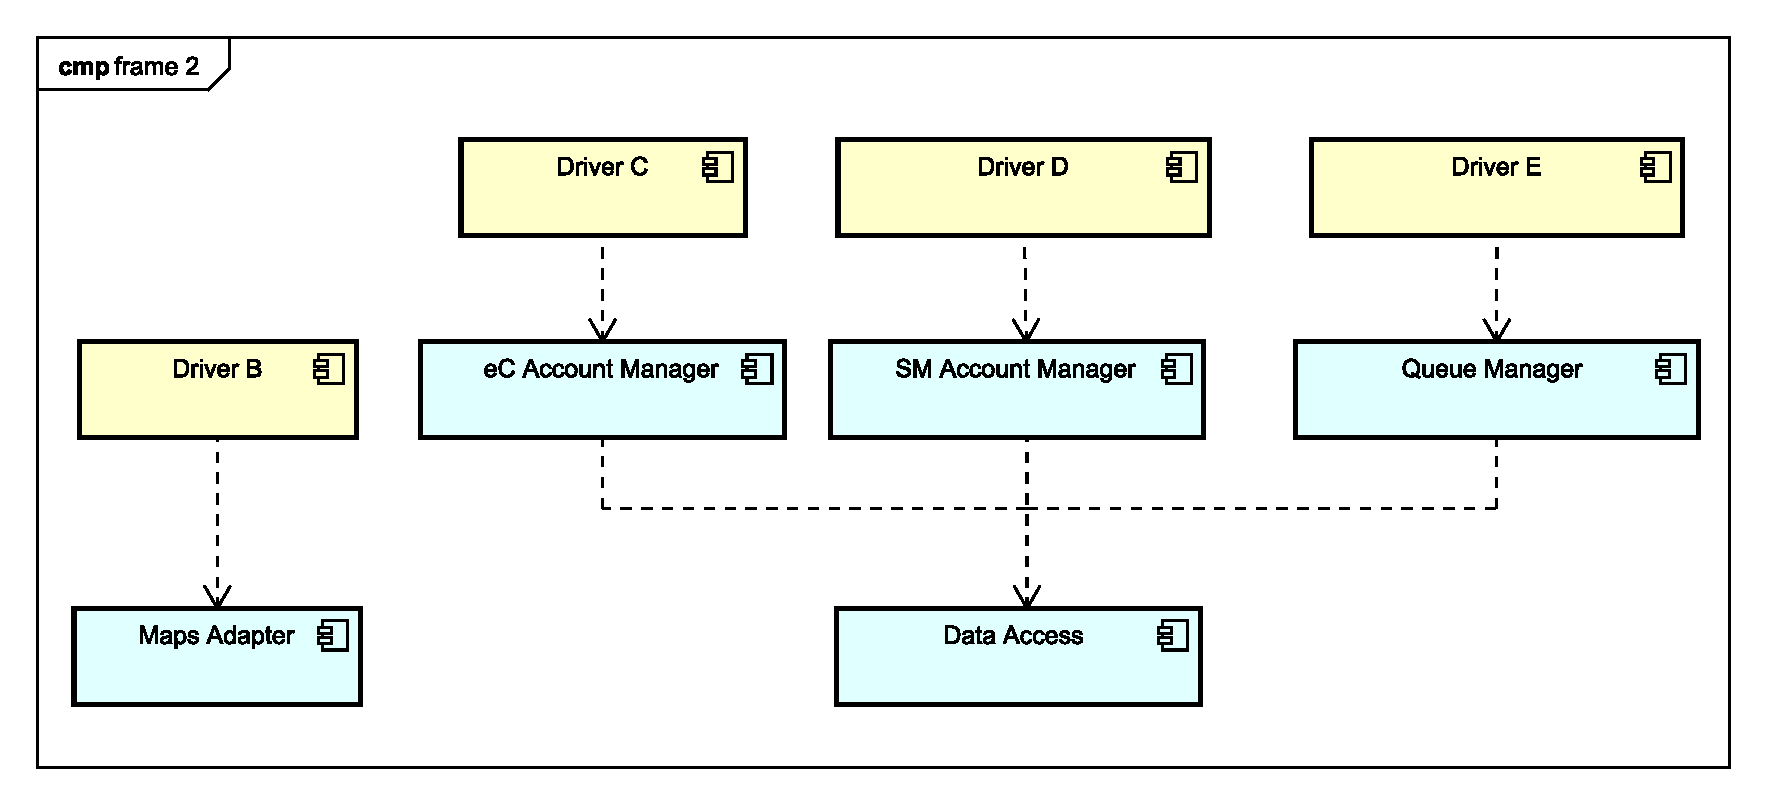
\includegraphics[width=\linewidth]{iit/frame_2}
		\caption{Adding some modules that use function provided by the Data Access and their drivers}
		\label{frame_2}
	\end{subfigure}
\end{figure}

\begin{figure}[h]
	\centering	
	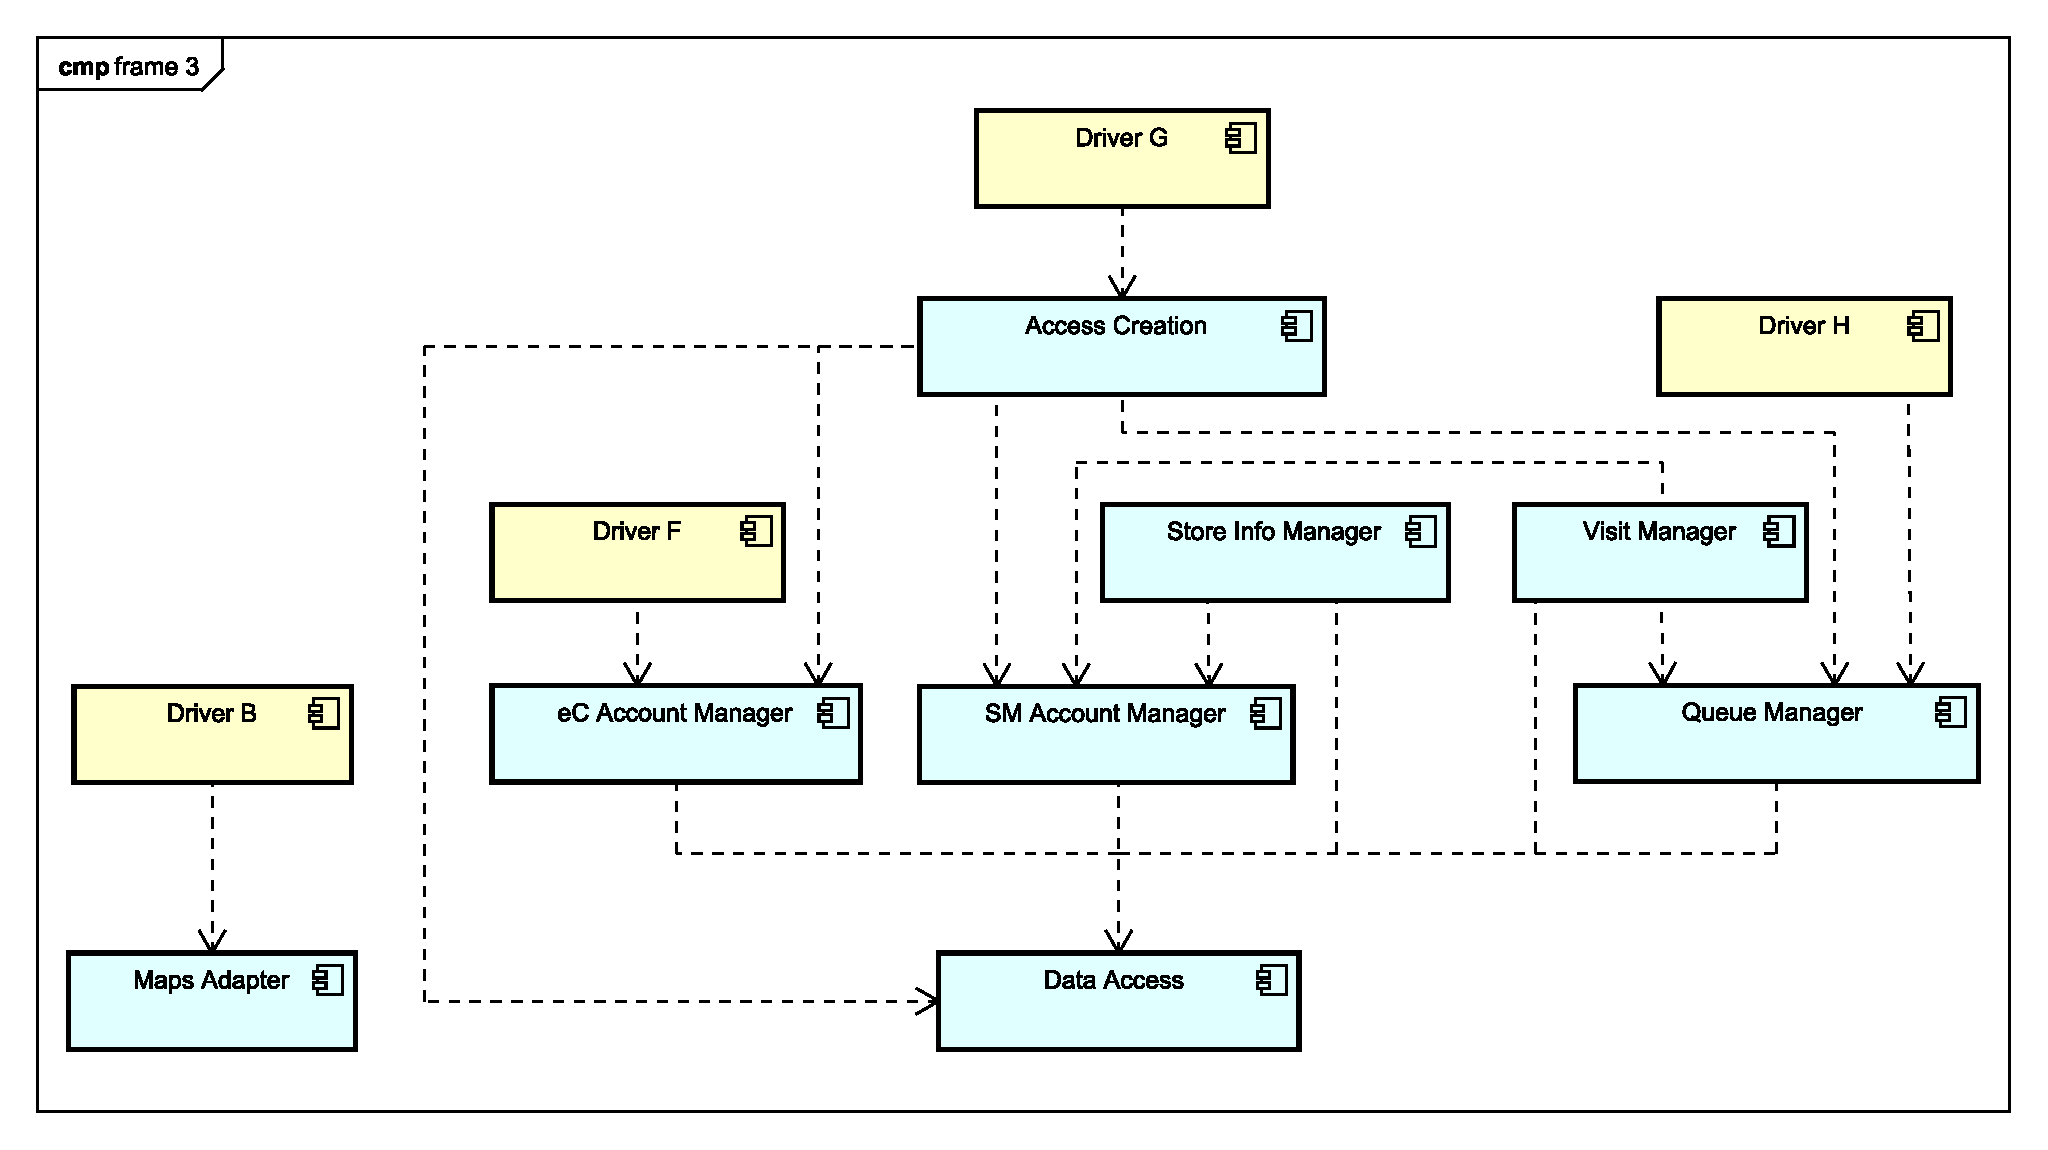
\includegraphics[width=\linewidth] {iit/frame_3}
	\caption{Realization of Access Creation, Store Info Manager, and Visit Modules}
	\label{frame_3} 
\end{figure}

\begin{figure}[p]
	\centering	
	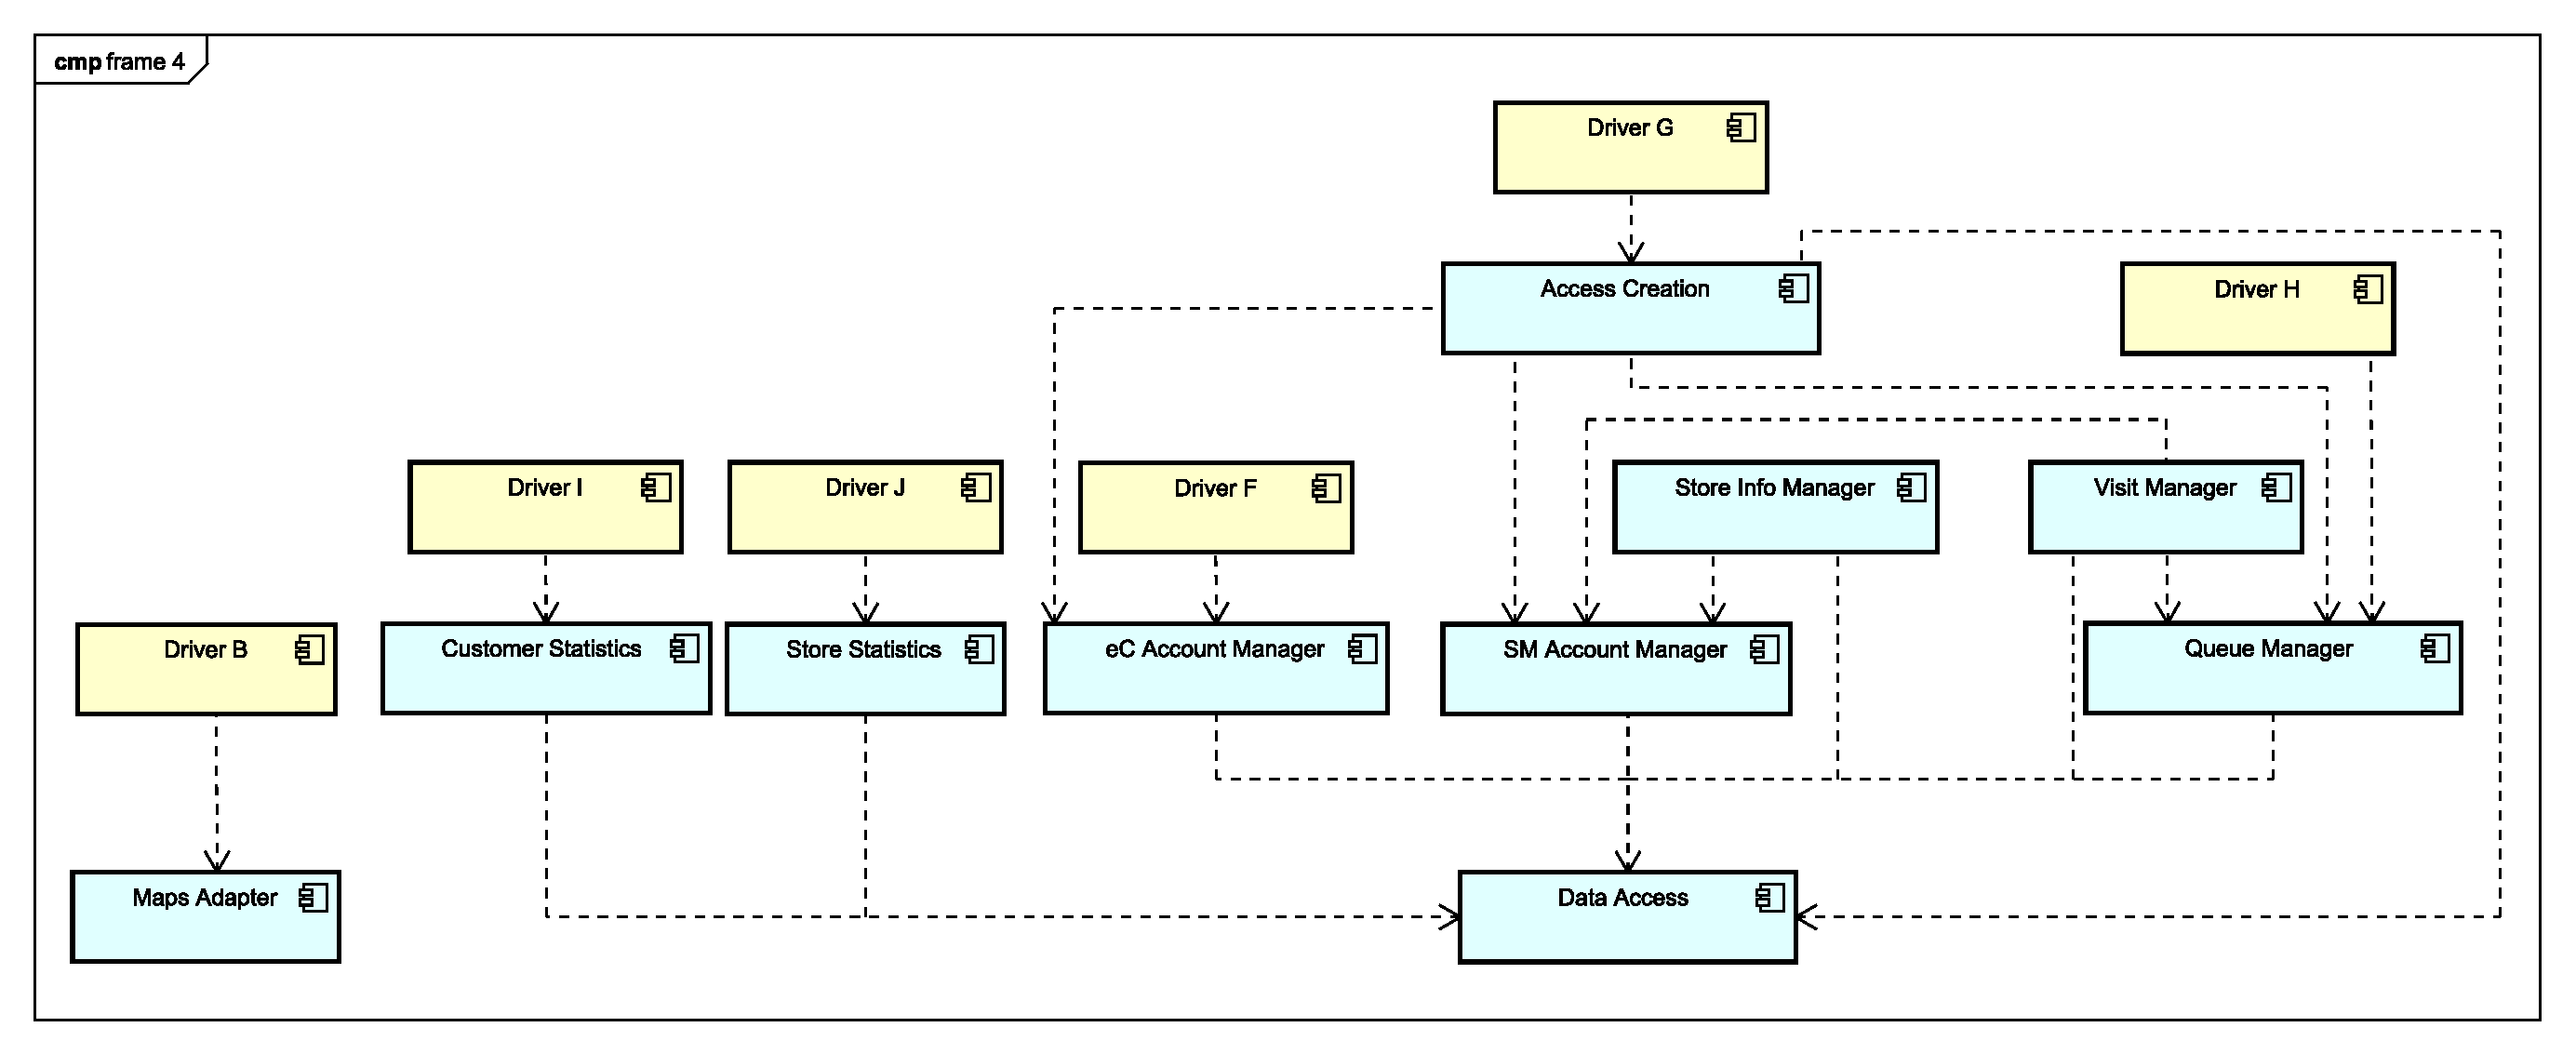
\includegraphics[width=\linewidth] {iit/frame_4}
	\caption{Implementation and integration of Statistics and Store Info Manager Modules}
	\label{frame_4} 

	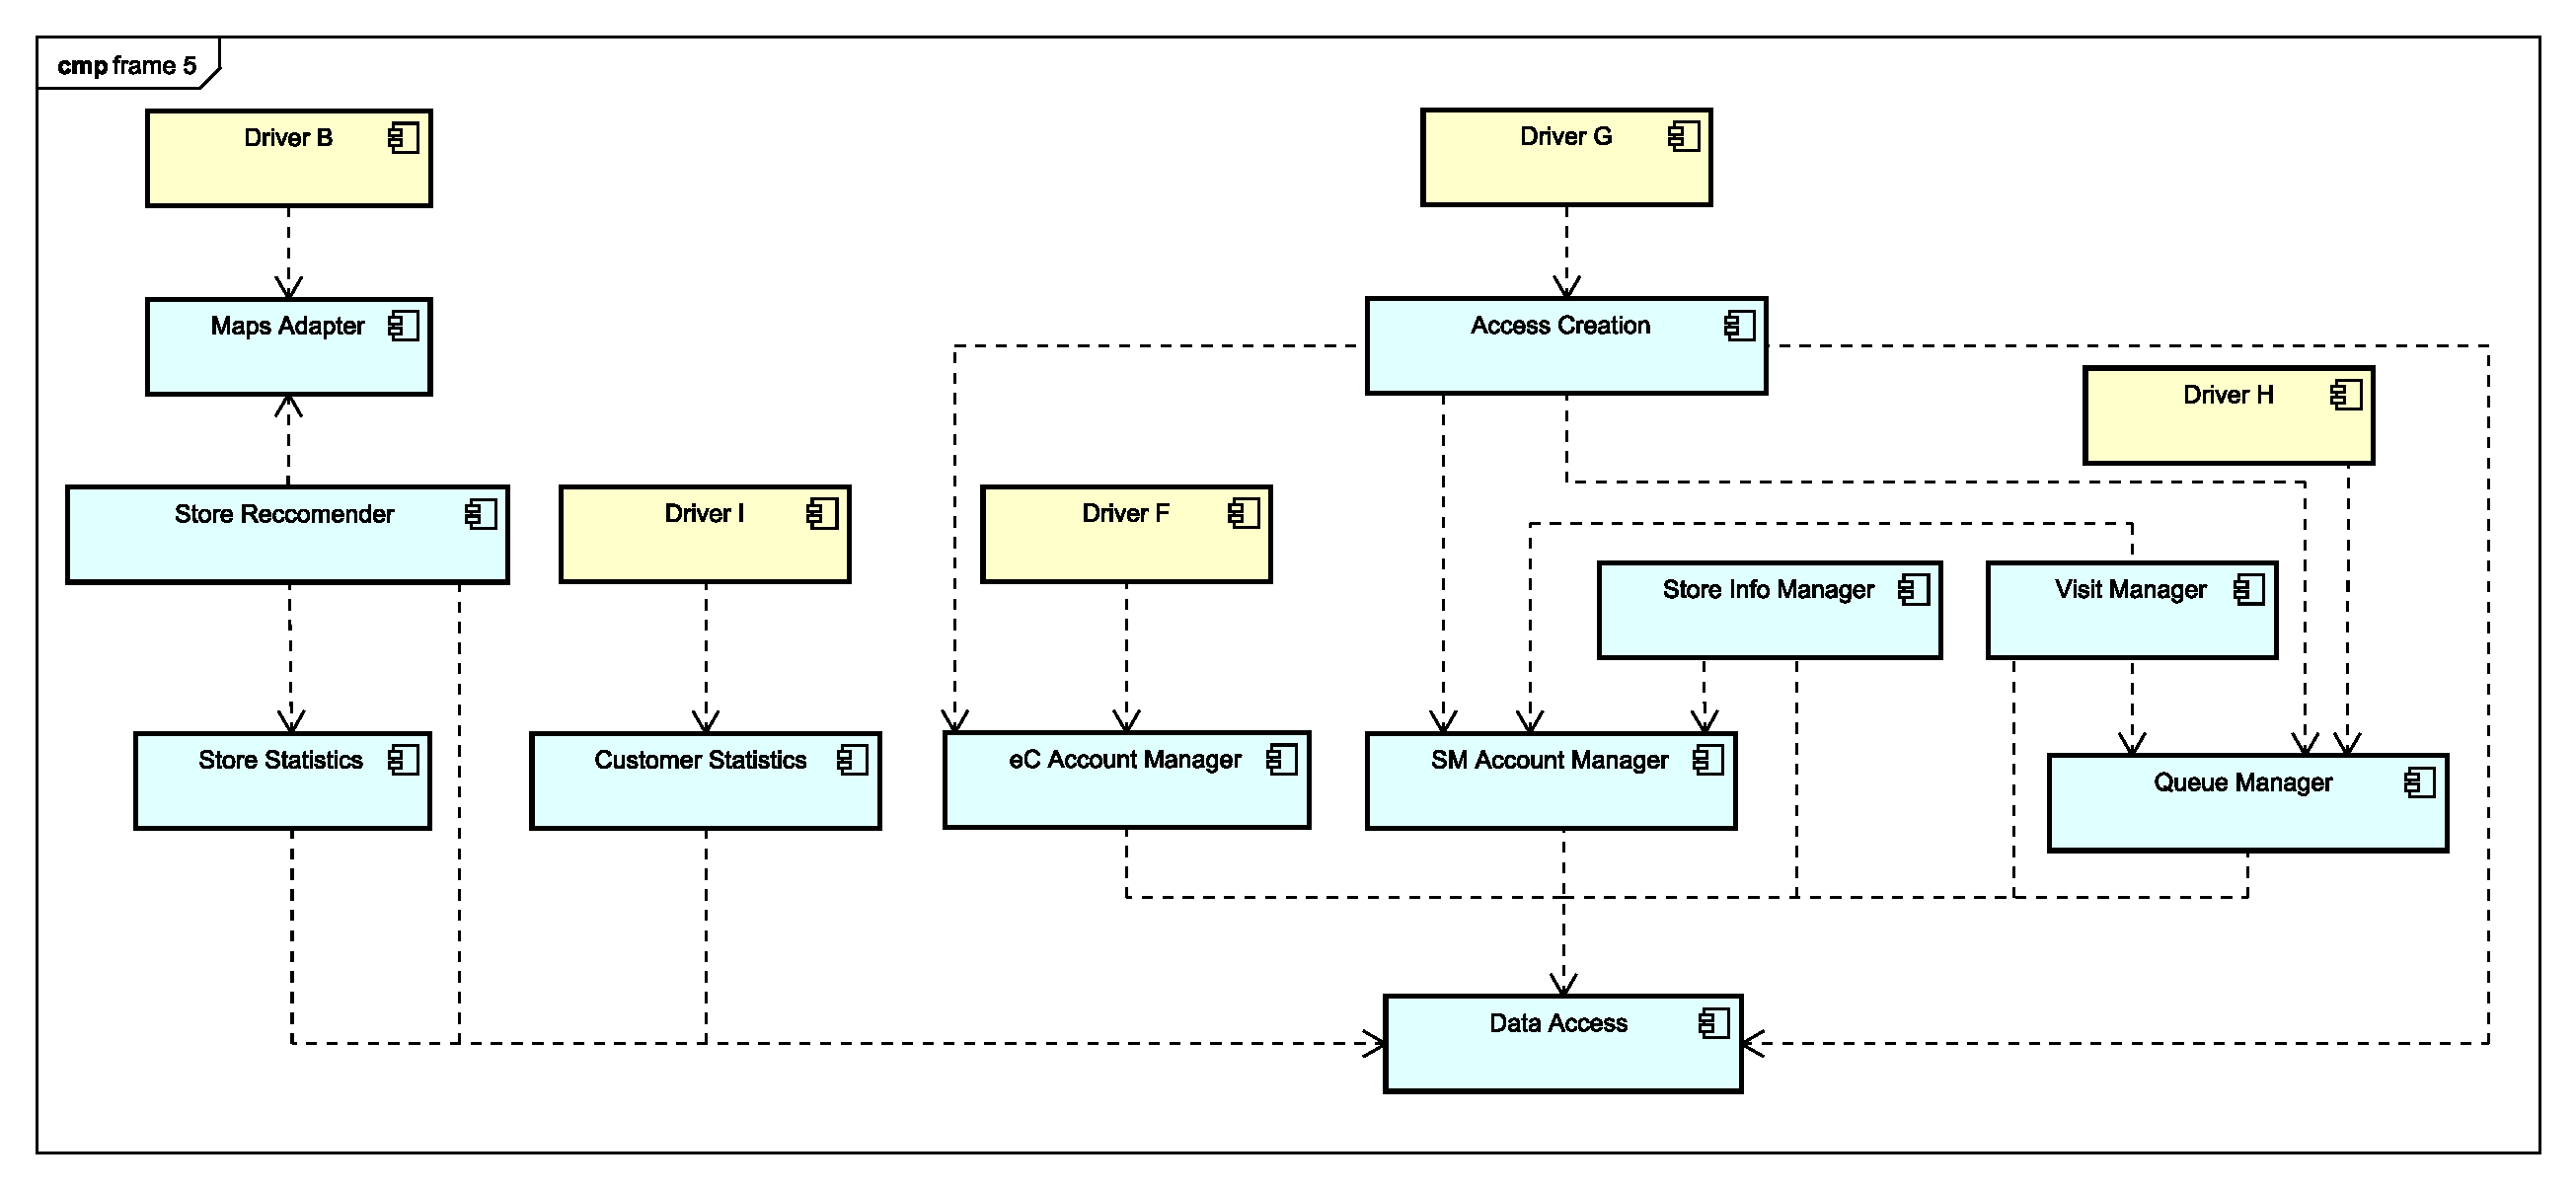
\includegraphics[width=\linewidth] {iit/frame_5}
	\caption{Adding the Store Recommender Module and integrating it with its dependencies}
	\label{frame_5} 

	\centering	
	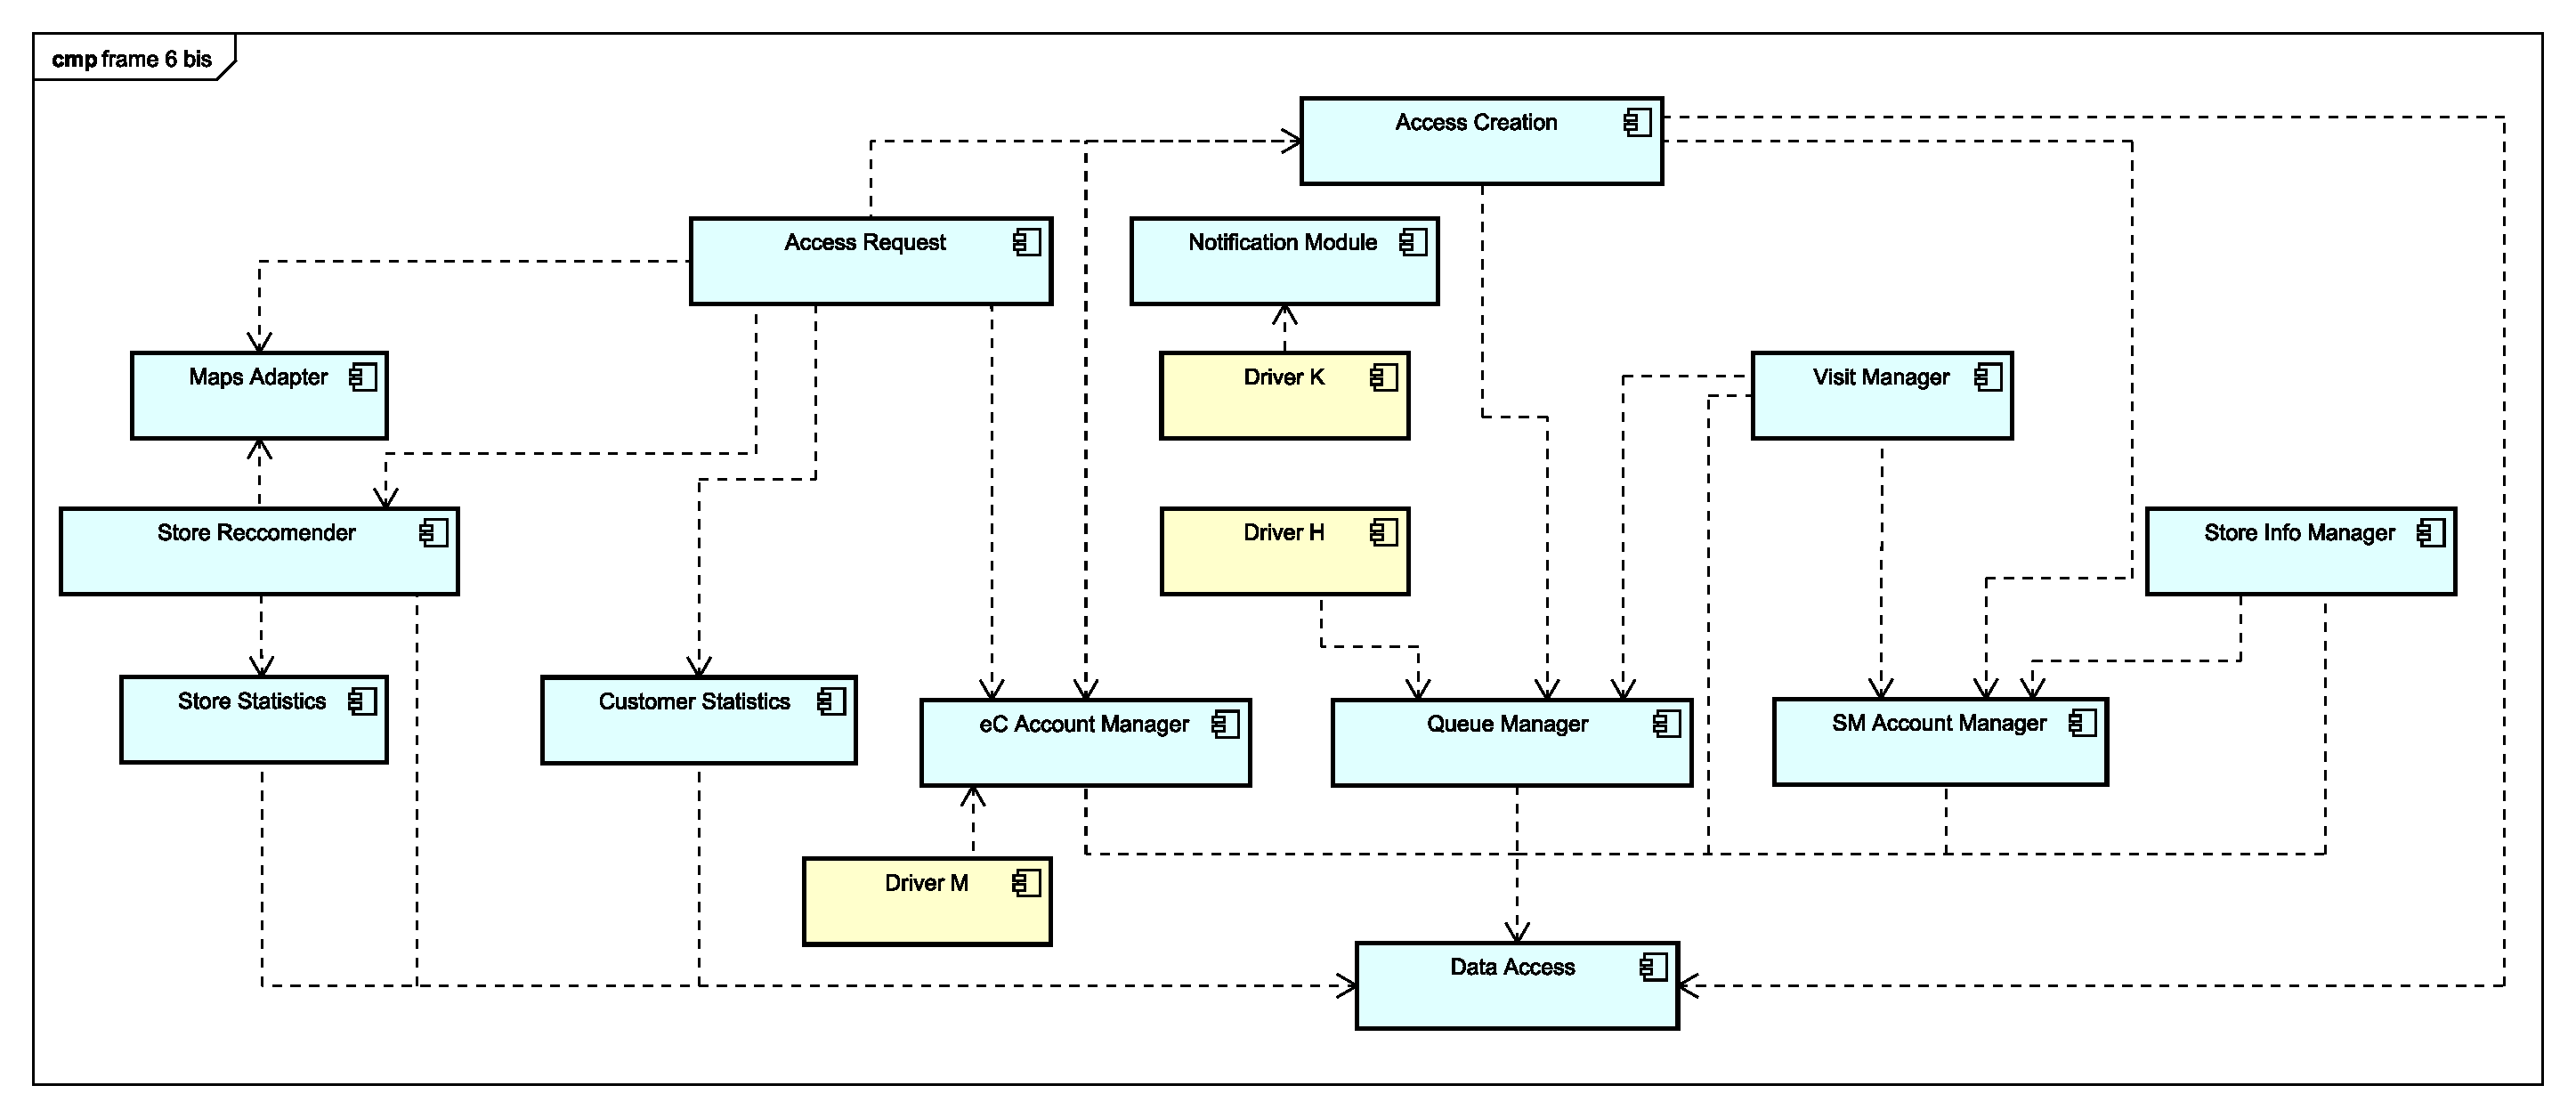
\includegraphics[width=\linewidth] {iit/frame_6}
	\caption{Integration of Access Request and Notification Modules}
	\label{frame_6} 
\end{figure}

\begin{figure}[h]
	\centering	
	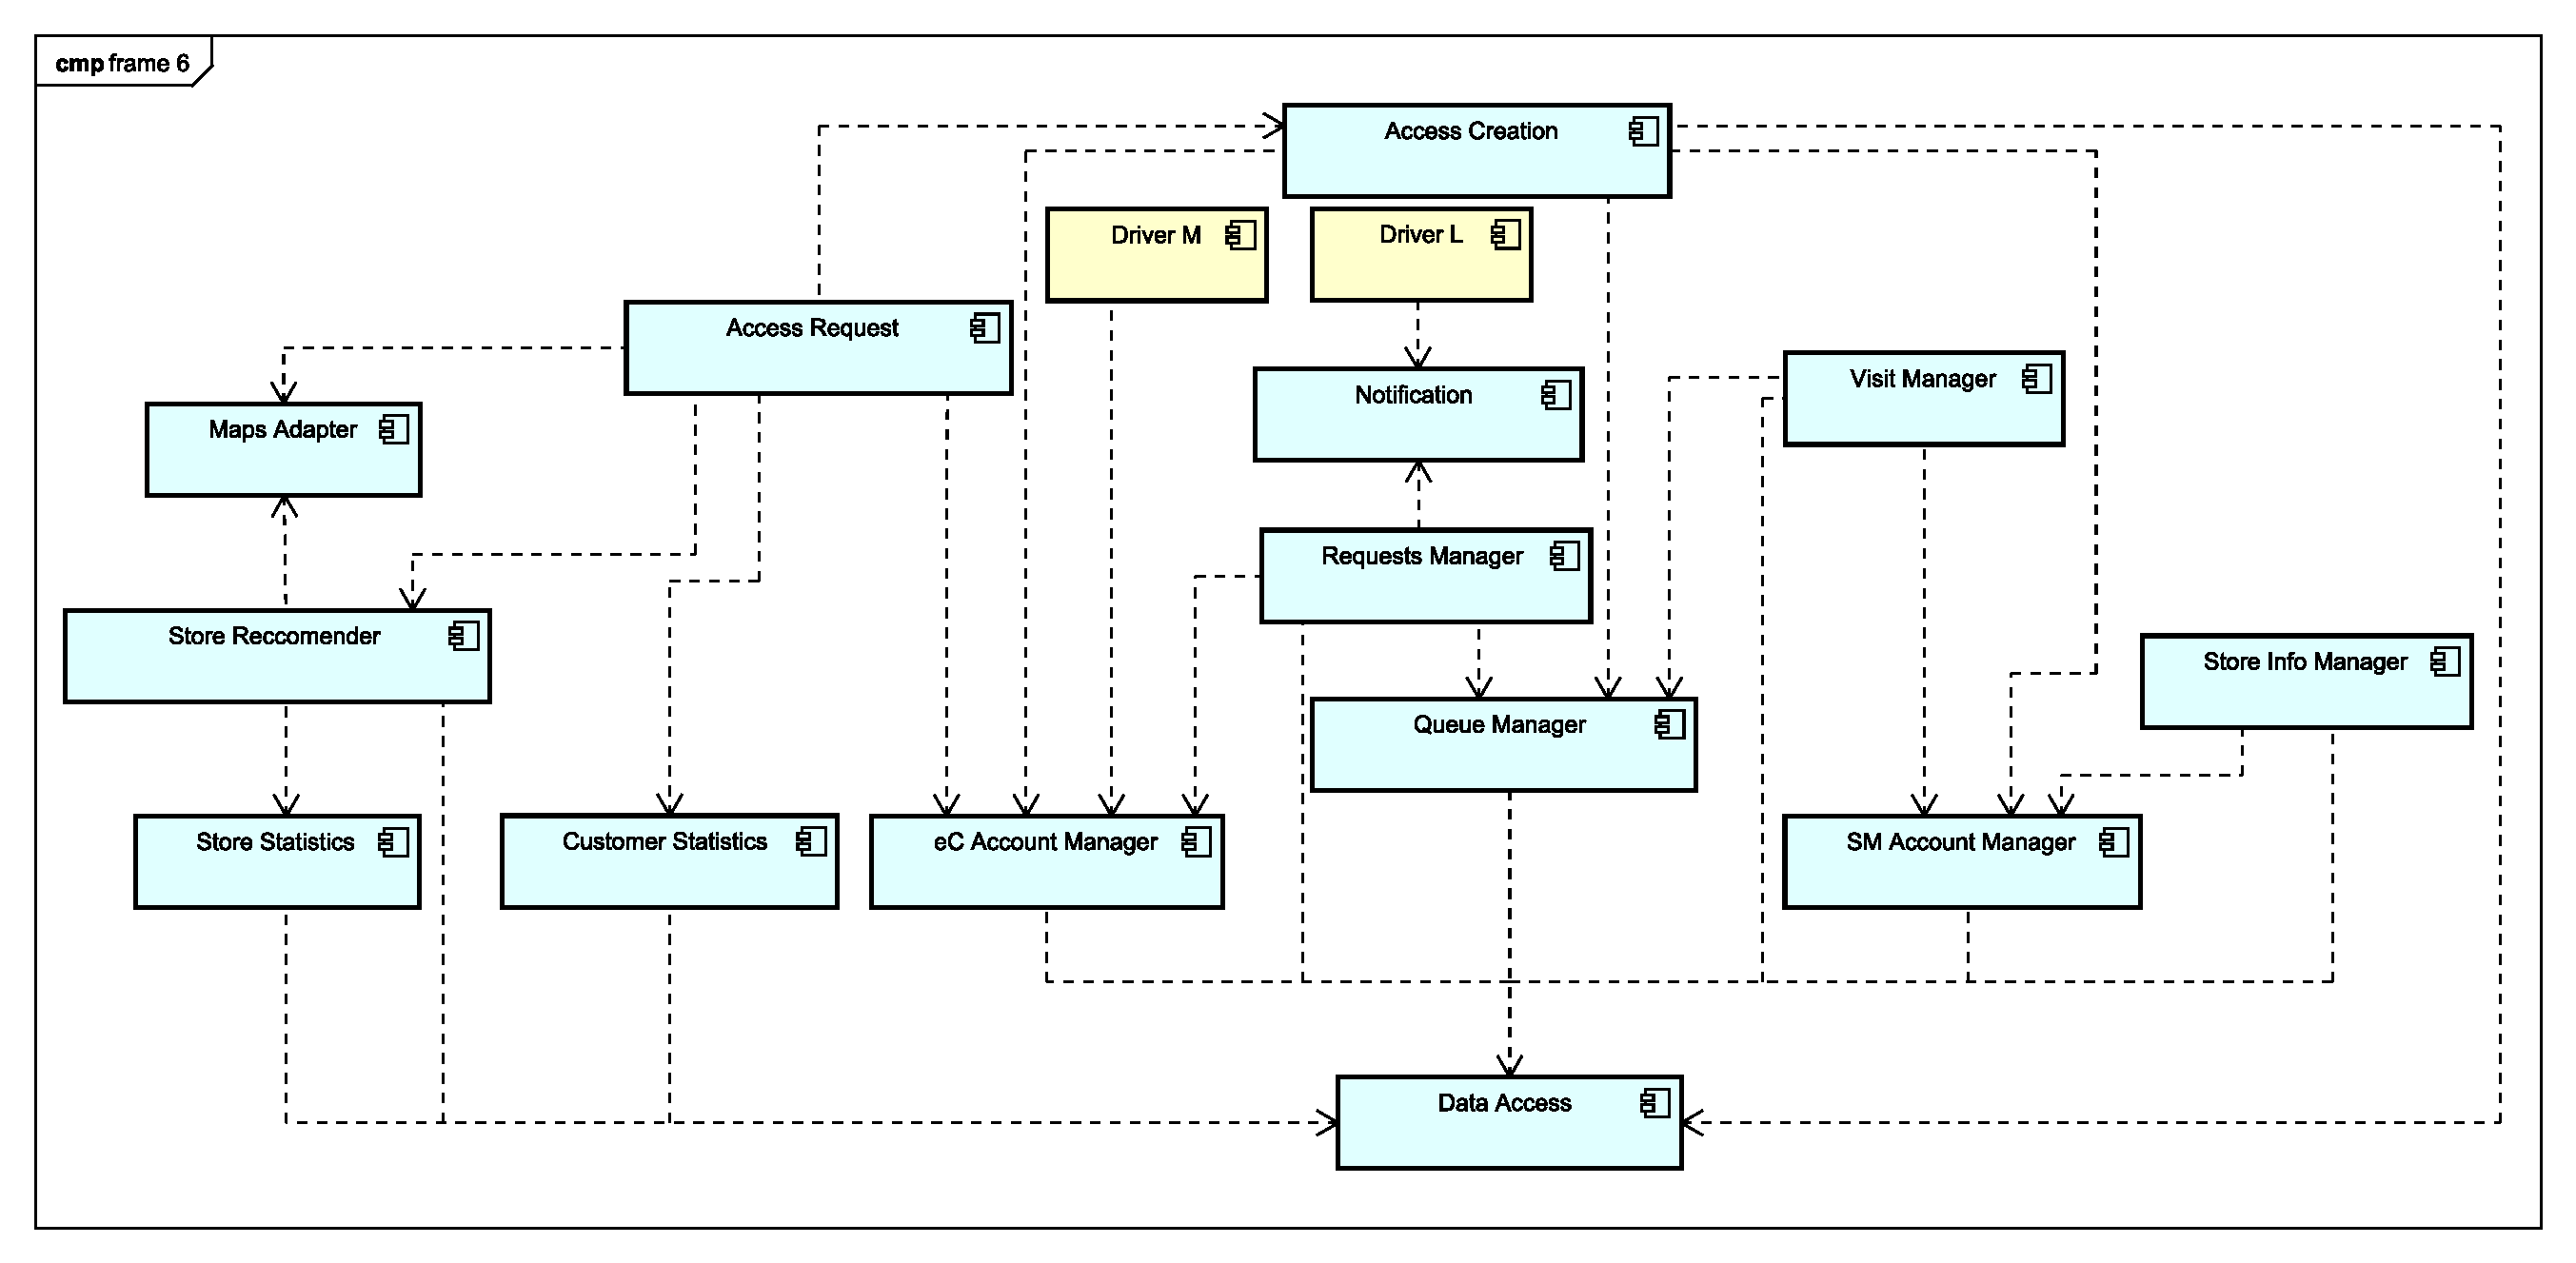
\includegraphics[width=\linewidth] {iit/frame_7}
	\caption{Addition of the Requests Manager Module}
	\label{frame_7} 
\end{figure}

\begin{figure}[h]
	\centering	
	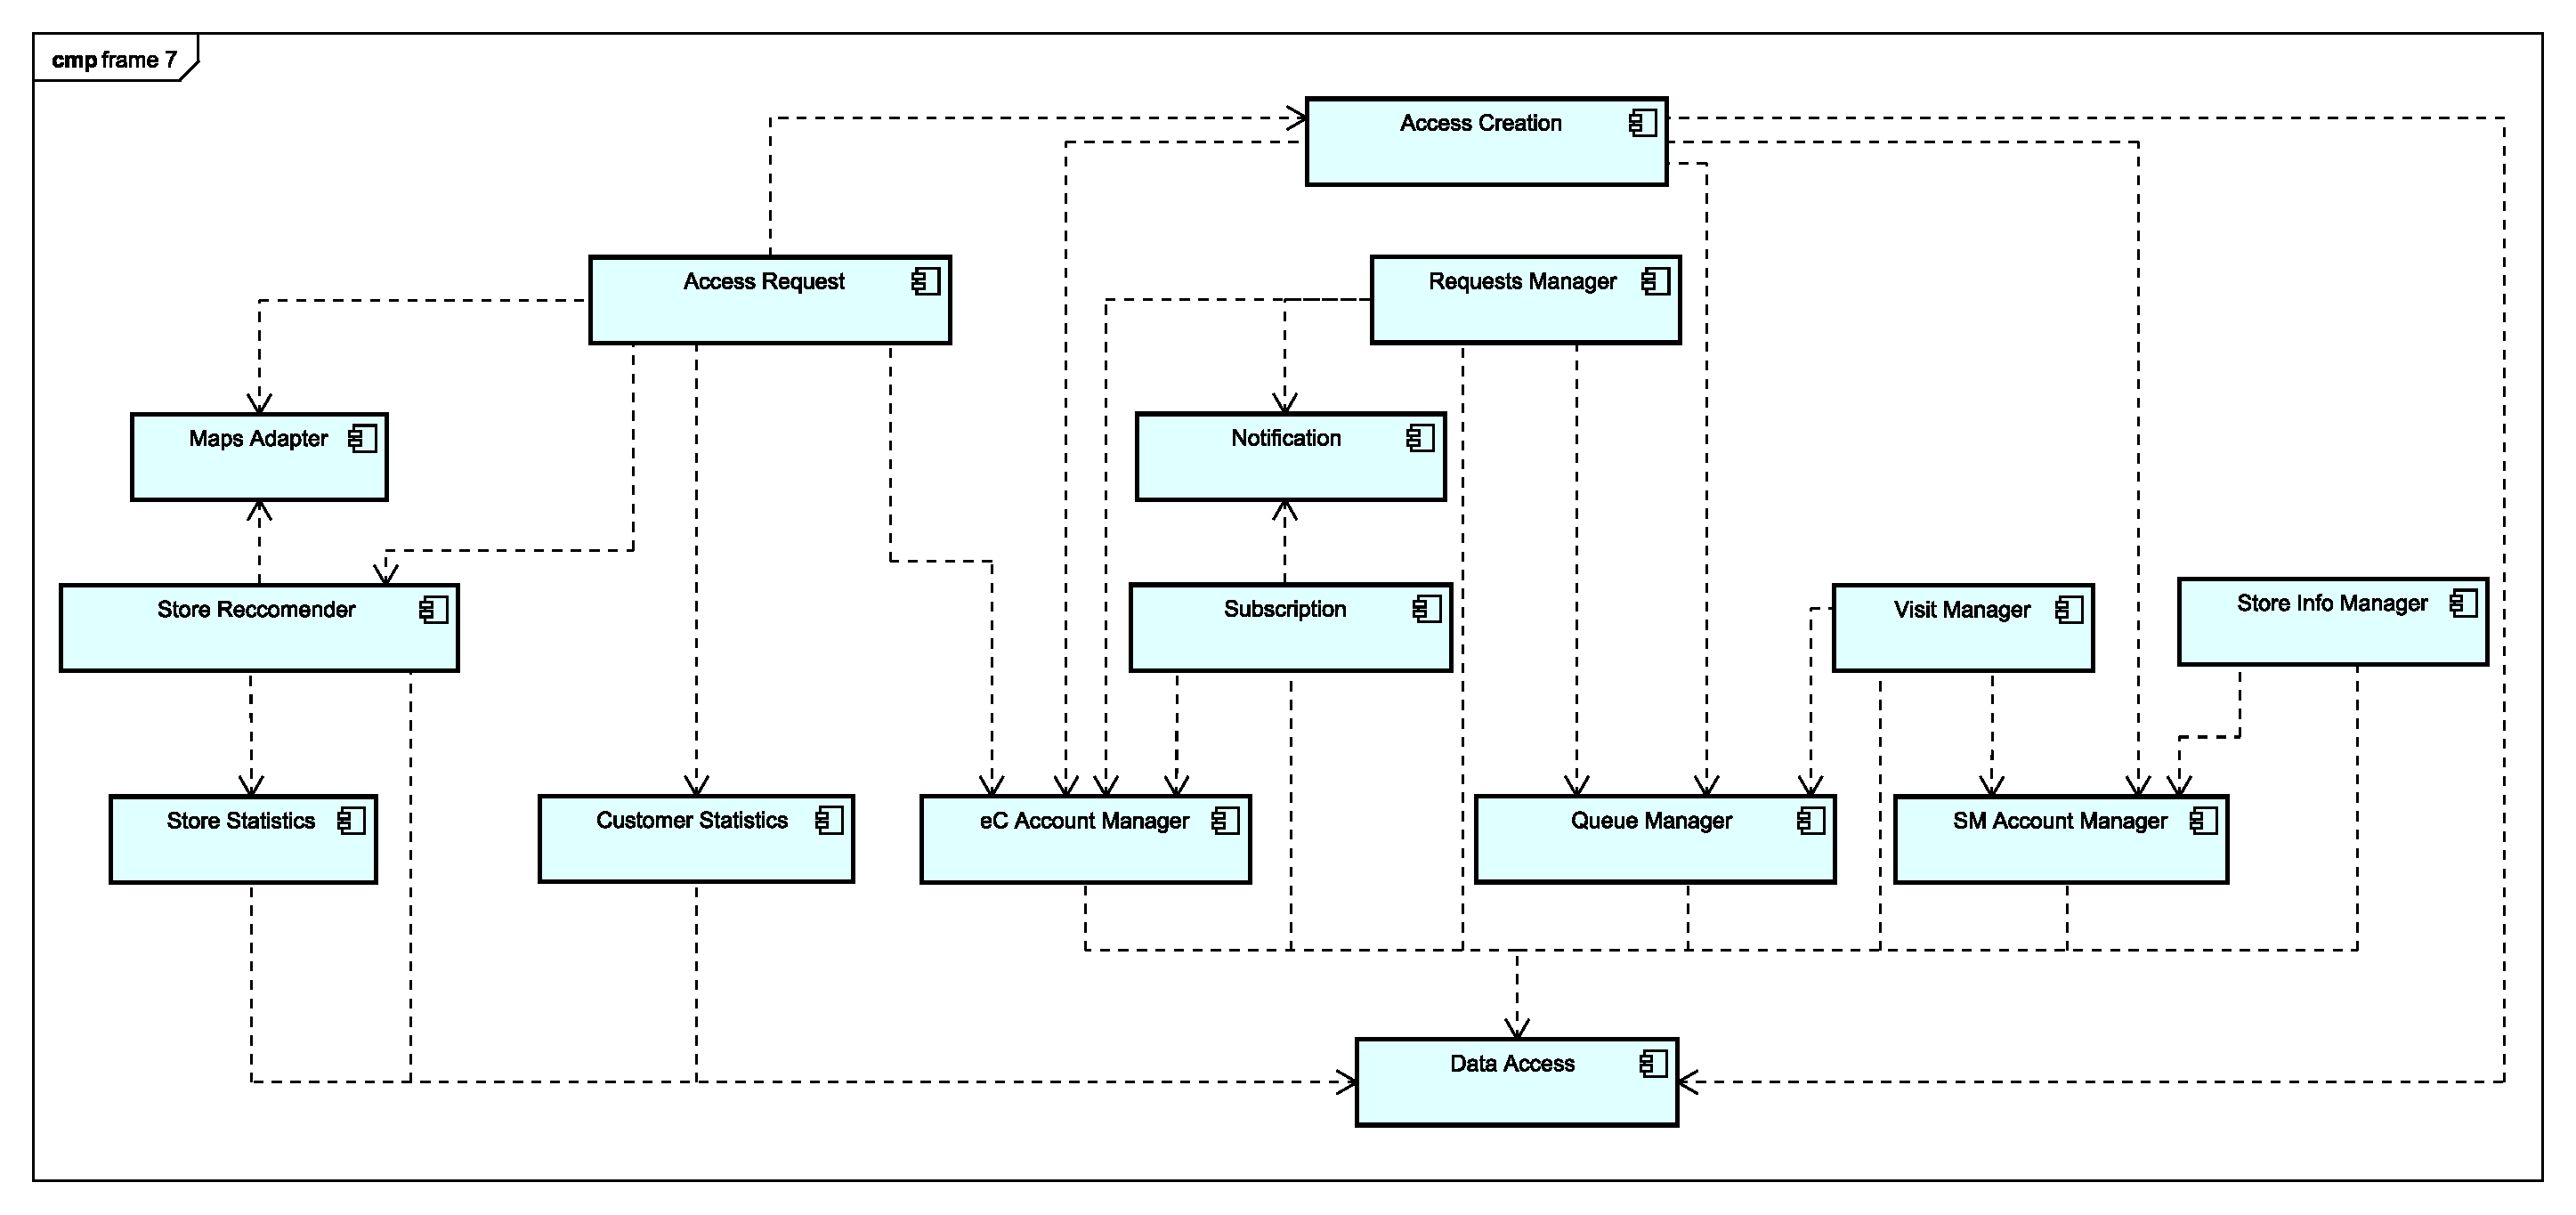
\includegraphics[width=\linewidth] {iit/frame_8}
	\caption{Final module integration with the previously missing Subscription Module}
	\label{frame_8} 
\end{figure}

\clearpage